\section*{Results}
\label{results}
%
The probability of choosing one stimuli over another is calculated for each comparison. The results for the probabilities is shown in \autoref{tab:prob}. 
%
\begin{table}[H]
\centering
\begin{tabular}{@{}llllllllllll@{}}
\toprule
Sounds     & No. & 1    & 2    & 3    & 4    & 5    & 6    & 7    & 8    & 9    & 10 \\ \midrule
Truck      & 1   & 0    & 0.15 & 0.27 & 0.75 & 0.93 & 0.08 & 0.48 & 0.10 & 0.40 & 0.55 \\
Brake      & 2   & 0.85 & 0    & 0.57 & 0.97 & 0.97 & 0.22 & 0.77 & 0.50 & 0.65 & 0.83 \\
Train      & 3   & 0.73 & 0.43 & 0    & 0.92 & 0.95 & 0.15 & 0.80 & 0.62 & 0.63 & 0.92 \\
Water      & 4   & 0.25 & 0.03 & 0.08 & 0    & 0.63 & 0.03 & 0.28 & 0.10 & 0.10 & 0.33 \\
Boat       & 5   & 0.07 & 0.03 & 0.05 & 0.37 & 0    & 0.05 & 0.10 & 0.05 & 0.05 & 0.20 \\
Jackhammer & 6   & 0.92 & 0.78 & 0.85 & 0.97 & 0.95 & 0    & 0.97 & 0.88 & 0.92 & 0.95 \\
Mower      & 7   & 0.52 & 0.23 & 0.20 & 0.72 & 0.90 & 0.03 & 0    & 0.27 & 0.28 & 0.68 \\
Crash      & 8   & 0.90 & 0.50 & 0.38 & 0.90 & 0.95 & 0.12 & 0.73 & 0    & 0.67 & 0.87 \\
Mixer      & 9   & 0.60 & 0.35 & 0.37 & 0.90 & 0.95 & 0.08 & 0.72 & 0.33 & 0    & 0.71 \\
Vent       & 10  & 0.45 & 0.17 & 0.08 & 0.67 & 0.80 & 0.05 & 0.32 & 0.13 & 0.28 & 0  \\ \bottomrule
\end{tabular}
\caption{The probability that one stimulus is chosen over another stimulus.}
\label{tab:prob}
\end{table} 
\noindent 
%
To find out how many times the stochastic transitivities is violated, each of the three types is investigated and the number of times there is a violation is counted. The results are shown in \autoref{tab:Stocha}. 
%
\begin{table}[H]
\centering
\begin{tabular}{@{}ll@{}}
\toprule
Stochastic transitivity     & Violations \\ \midrule
WST      & 2   \\
MST      & 3   \\
SST      & 25   \\ \bottomrule
\end{tabular}
\caption{Results for the number of violations of the three stochastic transitivities.}
\label{tab:Stocha}
\end{table} 
\noindent 
%
To check how good a fit the BTL-model is, a Chi-square test is conducted and the results is shown in \autoref{tab:Chi}. 

\begin{table}[H]
\centering
\begin{tabular}{@{}lll@{}}
\toprule
$\chi^{2}$     & Df & p-value \\ \midrule
38.1358      & 36  &  0.3725   \\ \bottomrule
\end{tabular}
\caption{Results from the Chi-square test.}
\label{tab:Chi}
\end{table} 

\noindent To understand what the analysis shows, the scale values and confidence intervals is plotted and shown in \autoref{fig:Confidens}. 

\begin{figure}[H]
\centering
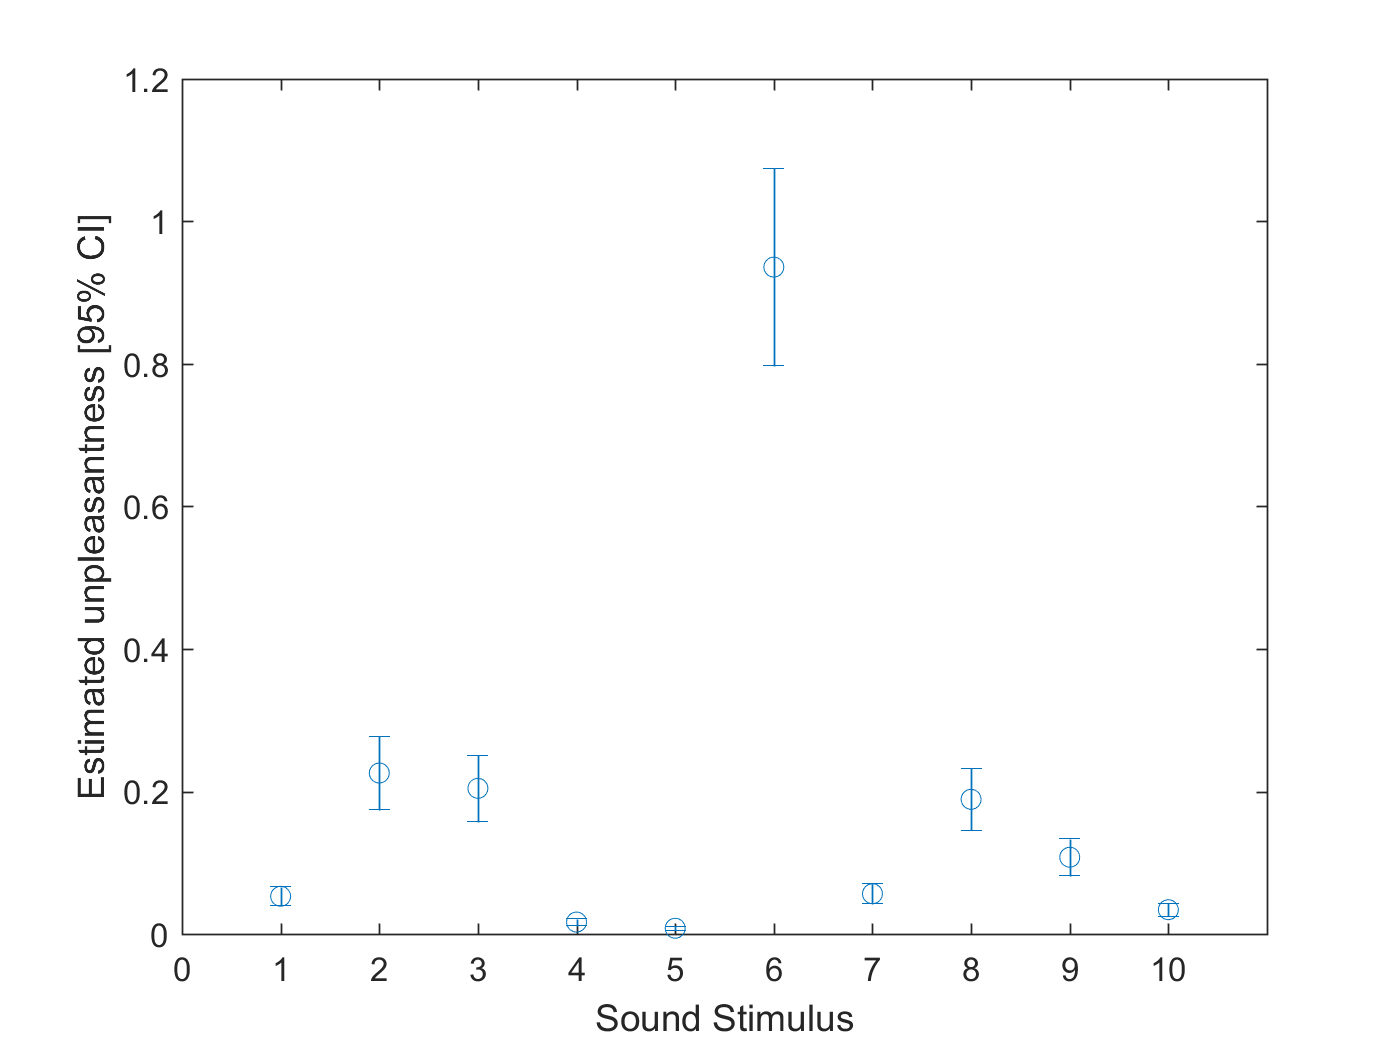
\includegraphics[width = 0.90\textwidth]{Figure/Confidens.png} 
\caption{Scale values and 95 \% confidence intervals}
\label{fig:Confidens}
\end{figure}